%%%%%%%%%%%%%% 18/02/2020 %%%%%%%%%%%%%%%% 
\subsection*{\textbf{18/02/2020}}
\subsubsection*{Days Aim}
\begin{itemize}
    \item Start to look at cross section
\end{itemize}

\subsubsection*{Day Summary}
\begin{itemize}
    \item Investigated background contributions from $ttbar_lep$, $Wplus_2lep$, and $Wminus_2lep$
    \item Calculated a preliminary value for $\sigma (Z \rightarrow ee)$ to be
    \subitem $\sigma (Z \rightarrow ee) = 1.943 nb$
\end{itemize}
%%%%%%%%%%%%% 9:00 %%%%%%%%%%%%%
\subsubsection*{09:00 - Lead BG}
Integrated Luminosity = $139 \text{fb}^{-1} (\pm 1.7\%)$

Coeficient $\epsilon$ given by sum of MC signal weights over that for relevent sample (found using TotExpected.Py) 

Made stacked plots for pTcone30 and etcone. Unexplained discrepancy of 2lep data aorund peak ~$0$MeV (Figure \ref{fig:2lep-Zee-Zmumu-Ztautau-fast_mean-etcone20_-2-5GeV_16-02-21_16-28}) 


Add ttbar\_lep to stack plots


$\epsilon_{\text{Zee}}$ = 19630128.89 

Quoted value for Zee cross section $76.0 \pm 0.8 \pm 2.0 \pm 2.6$ pb (https://arxiv.org/pdf/1212.4620.pdf)

%%%%%%%%%%%%% 10:38 %%%%%%%%%%%%%
\subsubsection*{10:38}

Rough estimate for the cross section: $\sigma (pp \rightarrow Z \rightarrow ee)$ is given by:
\begin{align}
    \sigma &= \frac{N^{selected} - N^{background}}{\epsilon \int L dt}
\end{align}
where
\begin{align}
     \epsilon &= \frac{\sum \text{weights for all MC events which pass selection cuts}}{\sum \text{weights for all events for that process}} 
\end{align}
For $Z \rightarrow ee$ use the cuts:
\begin{itemize}
    \item lep\_n = 2
    \item same flavour/type (lep\_type [0] == lep\_type[1])
    \item opposite charge (lep\_charge [0] != lep\_charge[1])
    \item invariant mass > 60 GeV 
    \subitem MC not modelled below this point
\end{itemize}
For $\sigma (pp \rightarrow Z \rightarrow ee)$:
\begin{itemize}
    \item $N^{selected} = 47531$
    \item $N^{background} = 0$
    \item $\epsilon = \frac{46740}{19630128.89} = $
    \item $\int L dt = 10.064 \textbf{fb}^{-1}$
\end{itemize}


cs = 1.9835391029941325e-09
\\
Other sources of background 
 - photon conversion 
 - hadronic jets
 -W or t decays can be detected as 2 electrons or muons when one is in fact a hadron jet or electron/moun from other source. 
 
%%%%%%%%%%%%% 14:00 %%%%%%%%%%%%%
\subsubsection*{14:00 - Lead DG - Number of leptons from W-plus and W-minus}
Investigating the decay paths of W-plus and W-minus.
\\
Plotting the number of leptons per event ($lep_n$)
\\
Cuts used in Fig.\ref{fig:14-00_18-02-21}:
\begin{lstlisting}
lepCut = "(" + "(lep_charge[0] != lep_charge[1]) && (lep_type[0] == lep_type[1]) && lep_n==2" + ")"

t.Draw("lep_n >> h_lep_n(100,0,100)", weighting + "*" + lepCut)
\end{lstlisting}
\begin{figure}[h!]
    \centering
    \begin{minipage}{0.5\textwidth}
        \centering
        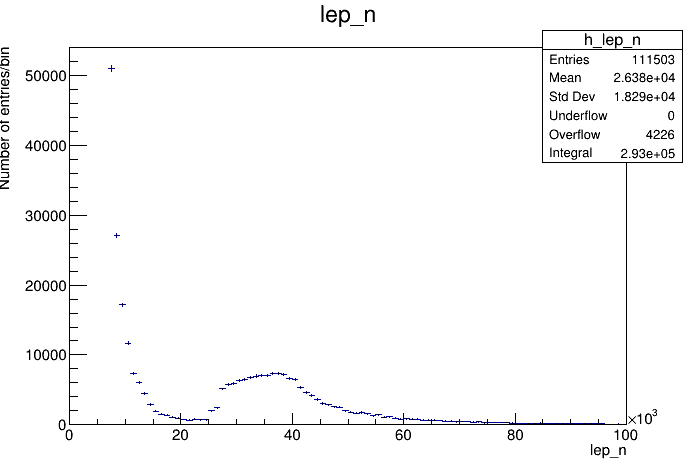
\includegraphics[width=\linewidth]{plots/18-02-2021/Wminus_2lep_lep_n_0-100_18-02-2021_14-12.png}
        (A)
    \end{minipage}\hfill
    \begin{minipage}{0.5\textwidth}
        \centering
        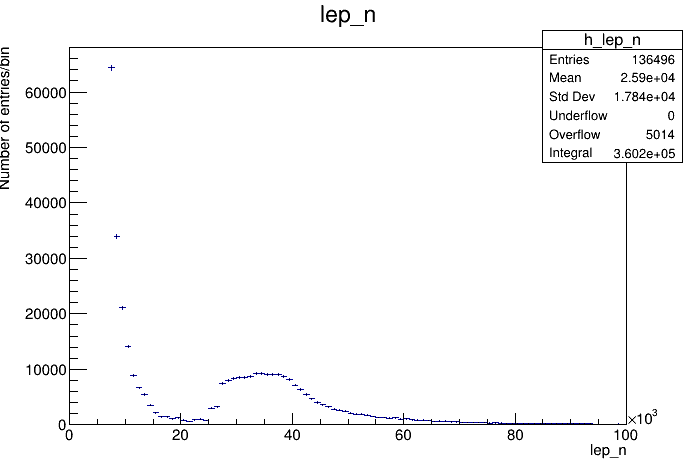
\includegraphics[width=\linewidth]{plots/18-02-2021/Wplus_2lep_slow_lep_n_0-100000_18-02-21_14-17.png}
        (B)
    \end{minipage}
    \caption{(A) Number of leptons in each event for Wminus-2lep. (B) Number of leptons in each event for Wplus-2lep. Cuts = basic: lepton pair with opposite charge and same type.}
    \label{fig:14-00_18-02-21}
\end{figure}
% (A) Wminus_2lep_lep_n_0-100_18-02-2021_14-12.png
% (B) Wplus_2lep_slow_lep_n_0-100000_18-02-21_14-17.png

There is an exponential decay in the number of leptons apart from a bump at about 35 leptons.
\\
This indicates that these leptons are most likely a result of lepton showers/jets.


%%%%%%%%%%%%% 14:40 %%%%%%%%%%%%%
\subsubsection*{14:40 - Invariant mass for Wplus-2lep and Wminus-2lep (Z -> ll)}
Plot the invariant mass between 60-150GeV for Wplus-2lep and Wminus-2lep for events that would look like $Z \rightarrow ll$.
\\
Large underflow, so increase range to 0-150 GeV 
\\
Still not totally decayed, increase range to 0-500 GeV.
\\
Cuts used in. Fig.\ref{fig:14-40_18-02-2021}:
\begin{lstlisting}
lepCut = "(" + "lep_n == 2 && (lep_charge[0] != lep_charge[1]) &&  (lep_type[0] == lep_type[1]) " + ")"

t.SetAlias("inv_mass_Zll","sqrt(2*lep_pt[0]*lep_pt[1]*(cosh(lep_eta[0]-lep_eta[1])-cos(lep_phi[0]-lep_phi[1])))")
  
t.Draw("inv_mass_Zll >> h_inv_mass(100,0,150e3)", weighting + "*" + lepCut)
\end{lstlisting}
\begin{figure}[h!]
    \centering
    \begin{minipage}{0.5\textwidth}
        \centering
        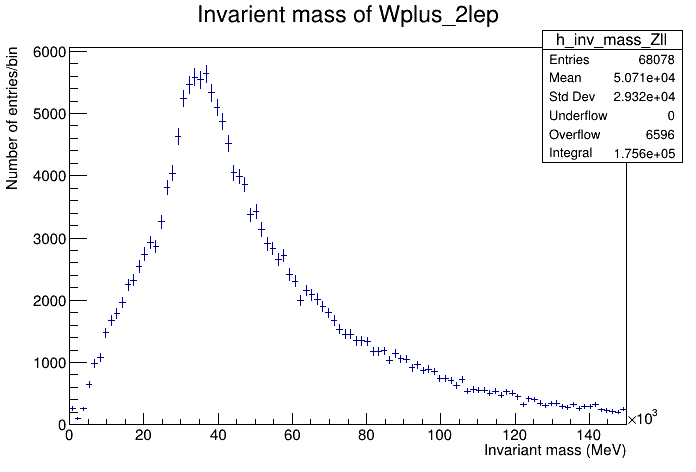
\includegraphics[width=\linewidth]{plots/18-02-2021/Invarient mass of Wplus_2lep 18-02-2021_14_49 .png}
        (A)
    \end{minipage}\hfill
    \begin{minipage}{0.5\textwidth}
        \centering
        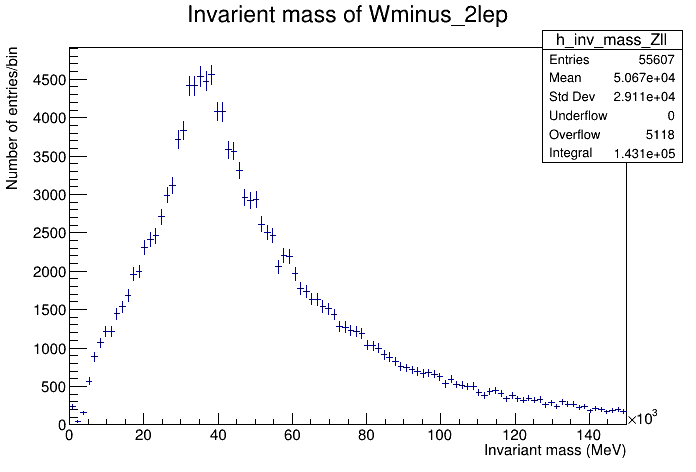
\includegraphics[width=\linewidth]{plots/18-02-2021/Wminus-2lep_invar-mass_18-02-21_14-54.png}
        (B)
    \end{minipage}
    \caption{(A) Invariant mass from Wplus-2lep (Background contribution) (B) Invariant mass from Wminus-2lep.  Cuts: (basic) lepton pair with oppsite charge and same type.}
    \label{fig:14-40_18-02-2021}
\end{figure}


%%%%%%%%%%%%% 16:10 %%%%%%%%%%%%%
\subsubsection*{16:00 - Lead BG - preliminary $\sigma (Z \rightarrow ee)$}
Finding the background contributions from $W^+ \rightarrow l\nu_l $ with the cut 
\begin{lstlisting}
     lepCut ="(" + "(lep_charge[0] != lep_charge[1]) && (lep_type[0]==11 && lep_type[1]==11) && lep_n==2 && (inv_mass_Zll > 60e3) && (inv_mass_Zll < 115e3)" + ")"
\end{lstlisting}
to select for e+e- pair.
\begin{align}
    N^{background}_{t\Bar{t}} &= 236276
    \\
    N^{background}_{W^+} &= 2247
    \\
    N^{background}_{W-} &= 1785
\end{align}
Sum of all weights for all MC events which pass cuts for Zee:
\begin{align*}
    = 4595000
\end{align*}
 
4817004

$\sigma(Z \rightarrow ee) = 1.94275964340403e-09 b$

//
TODO: 
\begin{itemize}
    \item Plot $ \Delta \phi$ 
    \item $\epsilon$ cut
\end{itemize}



